
\documentclass{IOS-Book-Article}

\usepackage{amssymb,amsmath}
\usepackage{bm}
\usepackage{dsfont}
\DeclareMathOperator*{\argmax}{arg\,max}
\DeclareMathOperator*{\argmin}{arg\,min}


\usepackage{mathptmx}
\usepackage{soul}\setuldepth{article}
\usepackage{graphicx}
\graphicspath{ {./figures/} }


\usepackage {multirow}
%\usepackage [english]{babel}
%\usepackage{setspace}
\usepackage{booktabs}
\usepackage{array}
\usepackage{tabularx}
%\usepackage{calc}
\usepackage{makecell}
\usepackage{array}
\newcolumntype{?}{!{\vrule width 1pt}}


%\usepackage{times}
%\normalfont
%\usepackage[T1]{fontenc}
%\usepackage[mtplusscr,mtbold]{mathtime}
%
\def\hb{\hbox to 11.5 cm{}}

\begin{document}

\pagestyle{headings}
\def\thepage{}
\begin{frontmatter}              % The preamble begins here.


%\pretitle{Pretitle}
\title{PICO to PICOS: Weak Supervision to Extend Datasets with New Labels}

%\markboth{}{April 2022\hb}
%\subtitle{Subtitle}
\author[A,B,C]{\fnms{Anjani} \snm{Dhrangadhariya}\orcid{0000-0003-1691-1338}%
\thanks{Corresponding Author: Anjani Dhrangadhariya, Informatics Institute, HES-SO Valais-Wallis, Technopole 3,
3960 Sierre, Switzerland; E-mail:
anjani.dhrangadhariya@hevs.ch.}},
\author[D]{\fnms{Gaetano} \snm{Manzo}}
and
\author[A,B]{\fnms{Henning} \snm{M\"uller}}

\runningauthor{A. Dhrangadhariya et al.}
\address[A]{Informatics Institute, HES-SO Valais-Wallis, Sierre, Switzerland}
\address[B]{University of Geneva (UNIGE), Geneva, Switzerland}
\address[C]{School of Health Sciences, HES-SO Valais-Wallis, Leukerbad, Switzerland}
\address[D]{Computational Health Research Branch, NLM, Bethesda, Maryland, USA.}
%
%
%
\begin{abstract}
Hand-labelling clinical corpora can be costly and inflexible, requiring re-annotation every time new classes need to be extracted.
PICO (Participant, Intervention, Comparator, Outcome) information extraction can expedite conducting systematic reviews to answer clinical questions.
However, PICO frequently extends to other entities such as Study type and design, trial context, and timeframe, necessitating manual re-annotation of existing corpora.
In this paper, we adapt Snorkel's weak supervision methodology to extend clinical corpora to new entities without extensive hand labelling.
Specifically, we enrich the EBM-PICO corpus with new entities through an example of ``Study type and design'' extraction.
Using weak supervision, we obtain programmatic labels on 4,081 EBM-PICO documents, achieving an F1-score of 85.02\% on the test set.
%We also propose a simple algorithm to map existing terminologies to weakly label an entity, which can be challenging, especially in clinical research with fuzzy entity definitions.
\end{abstract}

\begin{keyword}
weak supervision\sep information extraction\sep
clinical NLP
\end{keyword}
\end{frontmatter}
%\markboth{April 2022\hb}{April 2022\hb}
%\thispagestyle{empty}
%\pagestyle{empty}
%
%
%
\section{Introduction}
\label{sec:intro}
%
Clinical corpora, labelled by domain experts, serve specific purposes but such corpora are static and pose challenges in adaptability to new tasks. 
The resource consuming citation screening phase in systematic reviews (SRs) demands months of manual labor to analyze PICO data from clinical studies.
Despite the availability of the entity annotated corpus like EBM-PICO, manual analysis remains indispensable due to the complexity of additional information analysis such as study type and design, study context, and trial duration, essential for comprehensive evidence synthesis~\cite{methley2014pico}.



Weakly supervised (WS) information extraction (IE) techniques offer promise by programmatically labeling datasets using publicly-available sources like UMLS and NCBO BioPortal.
Fries \textit{et al.} 2021 used biomedical ontologies and regular expressions to train their WS system for extracting biomedical entities like diseases, chemicals, and drugs~\cite{fries2021ontology}. 
IE in the clinical domain is more challenging due to lack of standardization, language diversity, and fuzzy class definitions. 
Dhrangadhariya \textit{et al.} 2023 repurposed the weak supervision sources for the fuzzy, compositional PICO information but employed domain experts to do it~\cite{dhrangadhariya2023not}.
They did not tackle the challenge of extending a large corpus like EBM-PICO to new, relevant entities.
Inspired by prior efforts, our work pioneers weak supervision for enhancing hand-labelled datasets like EBM-PICO with new clinical entities~\cite{nye2018corpus}.
Leveraging weak supervision framework, we successfully label ``Study type and design'' across 4,081 EBM-PICO documents.
Evaluation using a 191 manually labeled documents confirms the efficacy of our approach, offering a pragmatic solution without relying on domain experts.
Our contribution expands the application of weakly supervised clinical IE, aiding faster SRs.
%
%
%
\section{Methods}
\label{sec:methods}
%
Figure~\ref{fig:approach} schematically represents our below-described approach.
%
%
%
\begin{figure*}[htb]
\centering
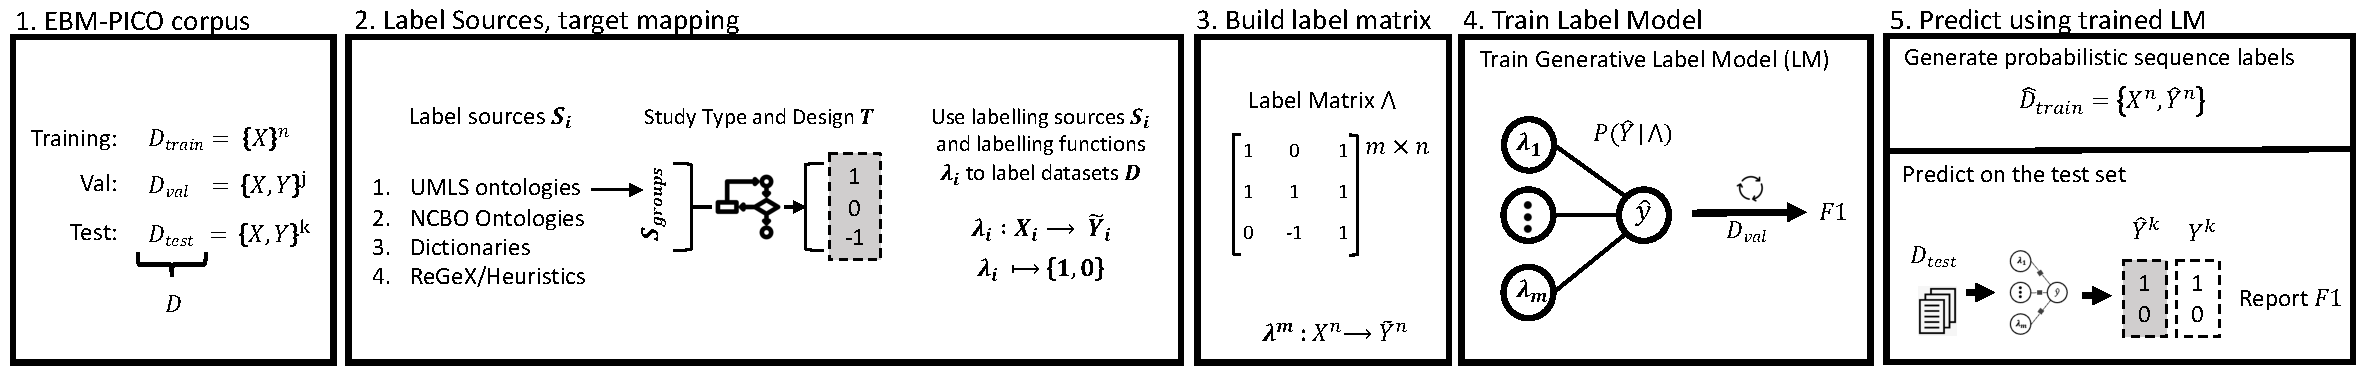
\includegraphics[width=0.99\textwidth]{Figures/approach.pdf}
\caption{WS approach: 1. Define the training, validation, and test sets. 2. Define labelling sources $S_{i}$. UMLS vocabularies are reused as labelling sources and mapped to the``Study type and design'' class labels. 3. LFs $\lambda_{i}$ map the training set to class labels using $S_{i}$ resulting in an $m \times n$ label matrix $\Lambda$. 4-5) The $\Lambda$ is used to train a generative LM that could be used to label unlabelled training sets with probabilistic labels.}
\label{fig:approach}
\end{figure*}
%
%
%

\paragraph{Dataset:} 
%
EBM-PICO was used to demonstrate the effectiveness of our approach.
It comes pre-divided into training (n=4,933) and test sets (n=191) for evaluation~\cite{nye2018corpus}.
The training set was further segmented into a validation set comprising $721$ documents.% ($\sim15\%$ of $4,933$).
After development of the annotation guidelines, the test set was doubly-annotated to calculate pairwise F1 measure as inter-annotator agreement (IAA)~\cite{deleger2012building}.
The IAA was $78.33\%$ and deeming it as sufficient, the validation set was singly annotated.
Hand-labelled validation and test sets are necessary for hyperparamter tuning and evaluation, respectively.
The training set was labelled using the weak supervision based programmatic labelling.
%
%
%
\subsection{Weak Supervision}
%
Weak supervision based programmatic labelling involves designing $m$ labelling functions (LF) $\lambda_{m}$, each of which is a function that takes input text sequence $X$ and a labelling source $s$ and produces an integer label sequence $\widetilde{Y} = (\widetilde{y_{1}}, \widetilde{y_{2}}, \ldots, \widetilde{y_{n}})$ ; $\widetilde{y_{i}} \subset \{1, 0, -1\}$.
We used programmatic labelling to label EBM-PICO training set with the ``Study type and Design'' class with the target labels $\widetilde{y_{i}}$.
The label $1$ represents ``Study type and design'' or positive class label, $0$ represents a negative class label, and $-1$ are abstains.
%The estimates $\hat{Y}$ of $Y$ are assigned as probabilistic token labels of $X$, leading to a weakly labelled dataset.
The ground truth $Y$ is latent and estimated by aggregating outputs from multiple LFs, resulting in $\hat{Y}$, which serves as probabilistic token labels for $X$, forming a weakly labelled EBM-PICO training set.
%
%
%
\paragraph{Labelling Sources:}
%
A labelling source $s$ can be a set of terms, expert-designed ReGeX, heuristics, or a combination of these sources that encode some domain-specific knowledge.
We used the 2021AB-full release of the UMLS Metathesaurus English subset after excluding zoonotic and non-English vocabularies, resulting in a pool of 112 vocabularies~\cite{humphreys1998unified}.
Labelling the ``Study type and design'' class entails using terms or concepts to represent this class by aligning the UMLS concepts onto the raw text EBM-PICO training set.
UMLS terms are organized under 127 internally-defined semantic groups $S_{groups} = (s_{group_{1}}, s_{group_{2}}, ..., s_{group_{n}});$ $n = 127$ like ``disease'', ``age group'', ``geographical location'' denoting whether a term represents a disease name or a location.
Semantic groupings impart meaning to the concepts and allow the repurposing of UMLS for programmatic labelling of related entities.
Our task was to map these $S_{groups}$ to the ``Study type and design'' class as per their representational value, ultimately mapping the concepts or terms to the class labels.



Non-UMLS ontologies like Clinical Trial Ontology\footnote{\url{https://bioportal.bioontology.org/ontologies/CTO}}, Randomized Controlled Trials Ontology\footnote{\url{https://bioportal.bioontology.org/ontologies/RCTONT}}, Ontology of Clinical Research\footnote{\url{https://bioportal.bioontology.org/ontologies/OCRE/}}, and Clinical Trials Ontology\footnote{\url{https://bioportal.bioontology.org/ontologies/CTONT/}} were used to represent $(+1)$ class labels.
Handcrafted dictionaries were designed using key-phrases from MeSH containing the generic term ``trial''.
The terms (e.g., ``quasi-experimental trial'', and ``crossover trial'') in this dictionary were used to label positive class labels.


We examined the most common keyword patterns in ``Study type and design'' class in the validation set.
These class-specific keyword patterns were used as ReGeX hooks along with the observed POS patterns to emit the positive class label.
For e.g., the trial design information ``double-blind, non-inferiority'' preceded the hook pattern ``randomized controlled trial''.
To identify such domain-specific patterns, a ReGeX was developed to identify the hook pattern ``randomized controlled trial'' and was combined with position and POS tags to identify preceding trial design information.
%
%
%
\paragraph{Source to Target mapping: }
The concepts in non-UMLS ontologies and the dictionaries were mapped to target label $+1$.
To map UMLS $S_{groups}$ to target label $+1$, we conducted a separate experiment using the validation set using the steps below:
%
%
%
\begin{enumerate}
    \item Label the hand-labelled validation set using all the UMLS $S_{groups}$.
    \item Calculate recall for the target label $+1$\footnote{The recall and the F1 score are binary metrics calculated for the ``Study type and design'' (positive) class.}.
    \item Rank and sort $S_{groups}$ based on their calculated recall.
    \item Next, label the validation set using the $S_{group}$ that ranked 1 ($S_{1}$) and calculate the initial recall $r$ and f1-score $f1$.
    \item Then loop through the ranked $S_{group}$ starting at rank 2 and sequentially add labels to the validation set (already labelled with $S_{group}$ rank 1) and calculate the new recall $r_{i}$ and f1-score $f1_{i}$ with the combined labels.
    \item After looping through all the $S_{groups}$, following heuristic was used to classify $S_{group}$ into representing either the positive ($+1$), negative ($0$) or abstain ($-1$) class. 
    We consider a $S_{group}$ representative of the ``Study type and design'' class (target label $+1$) if the change in the recall $\Delta r$ is $\geq1$  without impacting the f1-score. Such $S_{group}$ are marked as $+1$ and the rest as abstain or negative.
\end{enumerate}
%
%
%

%
%
%
\paragraph{LFs:}
%
We categorize our LFs into three types depending on the labelling sources.
An ontology or dictionary LF takes a set of terms (vocabularies, ontologies, \textit{etc.}) each mapped to one of $y \subset \{0, +1, -1\} $ class labels using heuristics.
A ReGeX LF used only regular expressions representative of the positive token label $\{+1\}$ and abstained from the rest.
A heuristic LF often took a generic ReGeX pattern, specific POS (part-of-speech) tag signals, and token positions to label tokens with the positive token class $\{+1\}$ labels and abstained from the rest.
%
%
%
\paragraph{Labelling and Label aggregation: }
%
Consider $S = (s_{1}, s_{2}, \ldots, s_{x})$ set of labelling sources used by $m$ LFs ($\lambda_{m} ;\Lambda = \{\lambda_{1}, \lambda_{2}, \dotso, \lambda_{m} \}$) to programmatically label the $X_{n}$ EBM-PICO training tokens to the aforementioned integer labels ($-1, 0, 1$).
The LFs map $X_{n}$ input tokens to the integer label sequence $\widetilde{Y}_{n}$ leading to a label matrix $\Lambda^{m \times n}$.
Majority voting (MV) and generative label model (LM) were tested to aggregate labels in $\Lambda^{m \times n}$.
%
%
%
\subsection{Experiments}
%
The experiments were carried out in seven tier and aimed to evaluate the impact of sequentially adding labelling sources on the label aggregation methods.
The tiers 1-4 tested the sequential addition of non-UMLS, dictionaries, and rule-based labelling sources to UMLS LFs in sequence.
Tier 5 examined whether up-weighting rules could improve performance, while tiers 6 and 7 measured the effect of removing non-UMLS and dictionaries from tier 4.
We evaluate performance using token-level macro F1, precision and recall over three runs of experiment tiers with three random seeds.
%xsWe used a CRF model trained on the hand-labelled validation set as the fully supervised (FS) baseline.
%
%
%
%\begin{table*}[!ht]
%    \centering
%    \begin{tabular}{c|c}
%        \hline
%        Tier & Labelling sources $s$ \\
%        \hline
%        1 & UMLS  \\
%        2 & UMLS + Non-UMLS  \\
%        3 & UMLS + Non-UMLS + dictionaries \\
%        4 & UMLS + Non-UMLS + dictionaries + ReGeX \\
%        5 & UMLS + Non-UMLS + dictionaries + weighted ReGeX (ReGeX $\times$ 2) \\
%        6 & UMLS + Non-UMLS + ReGeX - dictionaries \\
%        7 & UMLS + dictionaries + ReGeX - Non-UMLS \\
%        \hline
%    \end{tabular}
%    \vspace{1em}
%    \caption{The seven experiment tiers showing the labelling sources used by the programmatic labelling module.}
%    \label{tab:tiers}
%\end{table*}
%
%
%

%
%
%
\section{Results and Discussion}
\label{sec:results}
%

%
%
%
\begin{table*}[htb]
    \centering
    \begin{tabular}{l|l|r|r|r|r|r|r}
    \Xhline{1pt}
        & Experiments & \multicolumn{3}{c|}{MV} & \multicolumn{3}{c}{LM} \\ \Xhline{1pt}
        Tiers & LF tier & P & R & F1 & P & R & F1 (stdev) \\
        \Xhline{1pt}
        1 & UMLS & 48.64 & 50.00 & 49.31 & 61.03 & 56.42 & 58.02 (4.4 × $10^{-5}$) \\
        2 & + non UMLS & 51.58 & 50.01 & 49.37 & 50.21 & 50.02 & 49.62 (2.2 × $10^{-4}$)\\
        3 & + Dictionaries & 48.64 & 49.99 & 49.31 & 64.87 & 62.23 & 63.16 (3.6 × $10^{-2}$)\\
        4 & + Rules & 48.64 & 50.00 & 49.31 & 86.03 & 78.50 & 81.41 (4.2 × $10^{-3}$)\\
        5 & + Rules $\times$ 2 & 98.64 & 50.17 & 49.66 & 85.09 & 79.42 & 81.96 (7.4 × $10^{-3}$)\\
        6 & - Dictionaries & 98.64 & 50.13 & 49.59 & 81.40 & 72.55 & 75.37 (1.5 × $10^{-3}$)\\
        7 & - non UMLS & 96.22 & 53.31 & 55.56 & 89.96 & 81.41 & \textbf{85.02} (1.7 × $10^{-2}$)\\
    \Xhline{1pt}
    \end{tabular}
    \vspace{1em}
    \caption{\label{tab:res} Macro-averaged recall, precision and F1 \% for ``Study type and design'' extraction models. The best F1 score is shown in bold. Standard deviation (stdev) is reported for average over three runs.}
\end{table*}
%
%
%
Using the described labelling sources and functions, we developed a total of $144$ LFs: 112 UMLS LFs, 10 non-UMLS LFs, 2 dictionary LFs and 20 ReGeX LFs. 
The results of the experiments are listed in Table~\ref{tab:res}.
LF aggregation via MV fails to detect any meaningful signals and performs at a level close to or even worse than random.
For tier 7, however, removing non-UMLS LFs boosts the recall and therefore the F1 for MV.
The performance of UMLS alone for the LM tier 1 is poor.
Incorporating non-UMLS sources into the model results in a significant drop in F1 score by as much as $8.4\%$ again pointing towards the low representational value of this labelling source.
If a labelling source like non-UMLS sources, does not contain many of the terms that are representative of the entity in question, this could cause the F1 score to decrease upon their addition.
Our results prove this claim by conducting the ablation experiments.
The F1 score for the ``Study type and design'' entity deprecated on adding non-UMLS LF, suggesting that these functions were not typical for the ``Study type and design'' entity.
When non-UMLS labelling sources were removed from tier 7, a shoot-up in F1 score by 3.61\% from tier 4, where all the labelling sources were used.


The inclusion of dictionaries boosted the F1 by $13.52\%$, yet it plateaued at $63.16\%$
As expected, adding generic rules in tier 4 boosted the recall by $18.25\%$ from tier 1.
Up-weighting rule-based LFs in tier 5 led to a nominal F1 increase by 0.55\%.
In tier 6, removing handcrafted dictionaries decreases the previous best recall by $6.87\%$, demonstrating performance contribution.
In tier 7, removing the non-UMLS labelling sources improves the overall F1 by $3.06\%$.s% improving both recall and precision.
The utility and representational value of dictionaries are evidenced by a decrease of 6.05\% in the F1 upon their removal in tier 6.
%Removal of the dictionaries from the training LM resulted in a 6.04\% drop in the F1.
While ReGeX and heuristics designed for the ``Study type and design'' class may not be directly transferable to other entities, the methodology of developing ReGeX using hook patterns and a small labeled validation set can be effectively extended to other entity classes.
%The best performing weakly supervised LM in Tier 7 outperformed the fully supervised CRF model by 16\% on F1. 
%
%
%
%\section{Discussion}
%\label{sec:disc}
%
%
%
%
\section{Conclusion}
\label{sec:conclusion}
%
We adopted a weak supervision approach to enhance existing EBM-PICO dataset by incorporating additional categories, like ``Study type and design'' without relying on manual annotation. 
This is achieved through the application of weak supervision techniques using Snorkel.
Our approach achieved exceptional performance, with an F1 score of $85.05\%$ on the hand-labelled EBM-PICO test set, highlighting the potential of this method for rapidly generating large amounts of annotated data compared to traditional supervised approaches.
%We also provide a straightforward algorithm for mapping UMLS terms to entity classes, even in cases where expert guidance is unavailable, and semantic groupings are unclear.
The resources to reproduce this work are available on GitHub.
%
%
%
%%%%% References %%%%%
\bibliographystyle{spiebib} 
%
%
\bibliography{bibliography}
%
\end{document}
